% ShadowWeave workshop paper -- compressed 4-page version, NeurIPS 2026 style.
% Default (no option) = SUBMISSION mode: anonymized automatically + line numbers,
% which is what RoboWM's double-blind OpenReview review wants. For the de-anonymized
% camera-ready, switch to \usepackage[final]{neurips_2026}.
\documentclass{article}
\usepackage{neurips_2026}
% \usepackage[final]{neurips_2026}   % camera-ready

\usepackage[utf8]{inputenc}
% NOTE: no [T1]{fontenc} — this TeX Live lacks cm-super/lmodern, so T1 falls back to
% fuzzy bitmap PK fonts; default (OT1) Computer Modern stays fully vector.
\usepackage{graphicx}
\usepackage{booktabs}
\usepackage{amsmath}
\usepackage{microtype}
\usepackage[colorlinks=true,linkcolor=blue,citecolor=blue,urlcolor=blue]{hyperref}

\graphicspath{{../figures/}}

\title{ShadowWeave: Calibrated Amodal Occupancy Completion into Occluded Space from a Single Depth Frame}

% The style file anonymizes this automatically in submission mode.
\author{Kushaan Naskar\\
  University of Massachusetts Amherst\\
  \texttt{kushaannaskar@gmail.com}}

\begin{document}

\maketitle

\begin{abstract}
A mobile agent must reason about the space occluded by the very obstacles it navigates around
(``shadow''); we study how well a model can \textbf{complete} occupancy there from a
\textbf{single monocular-depth frame}, and whether it knows \emph{when it is guessing}.
ShadowWeave projects one depth frame into an egocentric bird's-eye-view (BEV) occupancy grid,
marks unobserved cells with an explicit shadow mask, and predicts occupancy and per-cell
uncertainty inside that mask. On a MuJoCo indoor benchmark, the model beats a persistence
baseline by a micro-averaged shadow-IoU gain of \textbf{+0.31 to +0.36 at a 5\,s horizon} (95\%
per-episode bootstrap CIs clear of zero at every horizon), far exceeds an observation-blind
dataset prior, and its uncertainty is \textbf{better calibrated inside shadow (ECE
0.043--0.047) than in directly observed space (0.058--0.086)}. A decomposition separating \emph{amodal completion} from \emph{temporal
forecasting} shows the gain is almost entirely completion; the pure-forecasting residual sits at
the noise floor. Randomizing room geometry per episode leaves
the gain statistically unchanged on never-seen rooms, ruling out memorization. The completed
grid and its uncertainty drive an eyes-free spatial-audio interface at 7\,ms (p95)
perception-to-planning latency; we release the methodology as a reusable protocol for honest
occupancy-completion claims.
\end{abstract}

\section{Introduction}
\label{sec:intro}

Agents --- a person entering a corridor, a robot rounding a shelf, a blind traveler crossing a
room --- act in space they cannot see; for safety-critical, eyes-free use, inference about that
space needs an honest estimate of its own reliability: a confident hallucination of clear space
behind a wall is worse than a calibrated ``I don't know.'' Prior work addresses parts of this problem but not their conjunction
(\S\ref{sec:related}).
\textbf{ShadowWeave} produces, from a single monocular-depth frame, (i) an egocentric BEV
occupancy grid, (ii) an explicit shadow mask marking cells the sensor cannot see, and (iii) a
calibrated per-cell occupancy probability inside that mask. Our contributions are:

\begin{itemize}\itemsep1pt\topsep1pt\parskip0pt\parsep1pt
\item \textbf{A calibrated amodal-completion result.} From one depth frame, the model completes occluded
  occupancy with a micro-averaged shadow gain of +0.31--0.36 at 5\,s (CIs clear of zero at every
  horizon), and its in-shadow uncertainty is \emph{better} calibrated (ECE 0.043--0.047) than in
  observed space --- the model conveys, not merely produces, hidden-space predictions.
\item \textbf{A decomposition methodology} that separates completion from forecasting. It reveals that the
  gain is spatial completion of persistent hidden structure; the pure-forecasting residual is at
  the noise floor (fixed static +0.000; moving tier +0.007 [+0.002, +0.012] at 5\,s ---
  significant but practically small, decaying with horizon as real forecasting should). We report
  this negative honestly: most pooled occupancy numbers in the literature share exactly this
  confound.
\item \textbf{A memorization confound-kill.} Randomizing room geometry per episode leaves the gain
  statistically unchanged on never-seen rooms (+0.306 fixed vs +0.309 [+0.294, +0.324]
  randomized), showing completion is per-scene inference, not a memorized layout.
\item \textbf{A real-time eyes-free system} that turns completed occupancy and its uncertainty into an
  A* path and nine-zone spatial-audio cues at 7\,ms p95 perception-to-planning latency.
\end{itemize}

\section{Method}
\label{sec:method}

\begin{figure}[t]
  \centering
  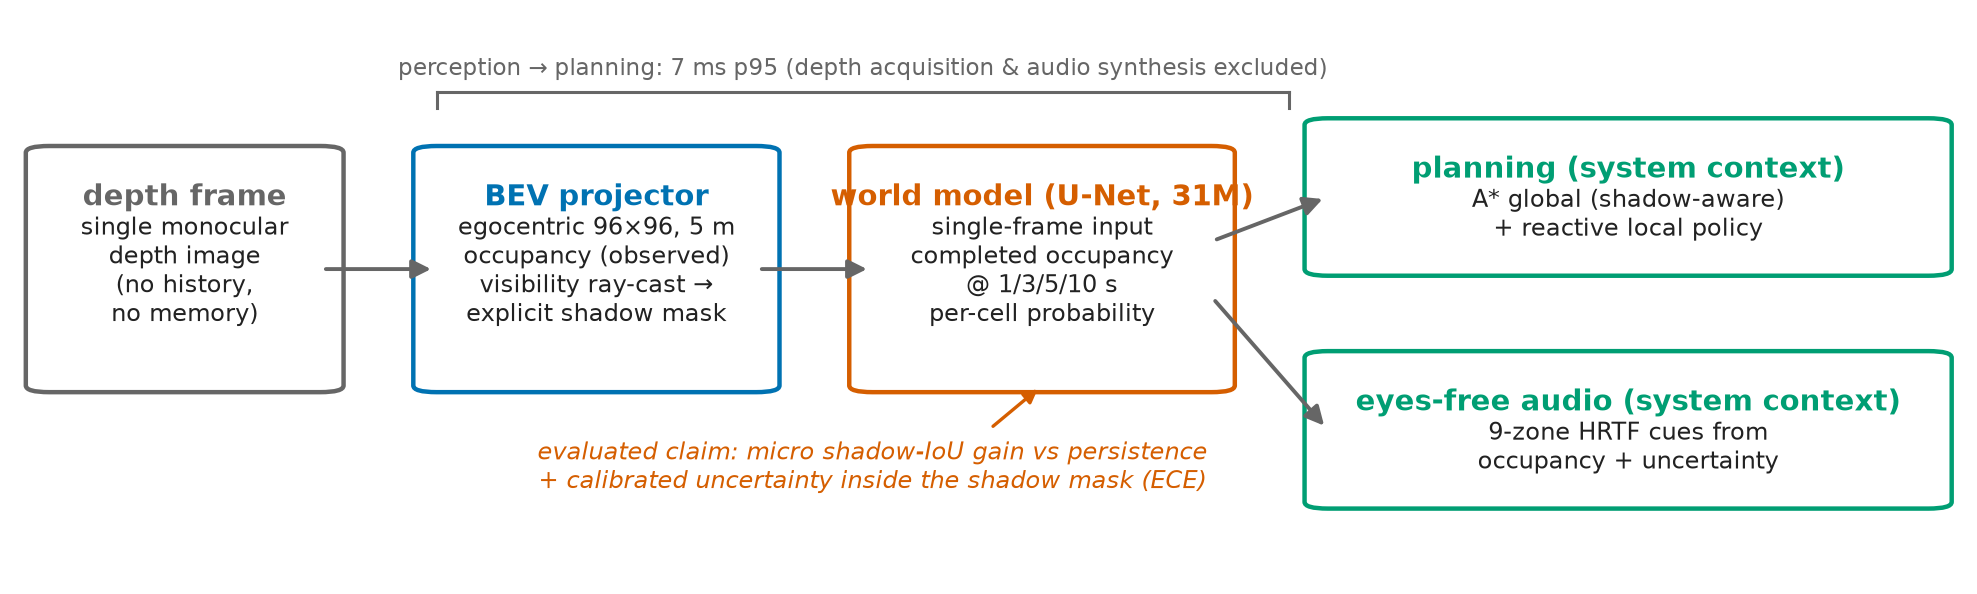
\includegraphics[width=0.52\linewidth]{architecture.png}
  \caption{Pipeline: depth frame $\to$ $96\times96$ egocentric BEV occupancy and visibility;
  thresholded visibility gives the shadow mask; a 31M U-Net predicts occupancy at 1/3/5/10\,s
  inside it, feeding A* planning and nine-zone HRTF audio.}
  \label{fig:architecture}
  \vspace{-8pt}
\end{figure}

A differentiable projector (Fig.~\ref{fig:architecture}) lifts each monocular-depth image
(rendered in simulation; from a monocular-depth network in deployment)
into an egocentric $96\times96$ BEV occupancy grid covering 5\,m ahead, plus a
\textbf{visibility} grid: cells along a ray up to the first returned surface are observed-free,
the surface cell observed-occupied, and everything beyond is \textbf{shadow}. Thresholding
visibility at 0.5 yields the shadow mask --- the region of interest for every metric here;
optical flow between BEV frames is an optional channel. A
31M-parameter U-Net predicts occupancy from the single-frame BEV stack at 1/3/5/10\,s as
per-cell probabilities, trained with positive-up-weighted binary cross-entropy (BEV targets are
$\approx$7\% occupied) on 400 episodes with early stopping and EMA weights; we report the
epoch-8 checkpoint (val.\ loss 0.300, IoU@5s 0.665). The input is a \textbf{single frame} with
no multi-frame memory, making the completion-vs-forecasting distinction
(\S\ref{sec:methodology}) sharp. The per-cell probability \emph{is} the uncertainty estimate; we
test calibration \textbf{inside the shadow region specifically}, not merely grid-wide (where
easy free space dominates). Downstream, the completed grid and its
uncertainty drive an A* planner (extra cost through unobserved cells), a reactive
collision-avoidance policy, and nine-zone HRTF audio cues; the audio interface is a
demonstration, not user-evaluated.

\section{Evaluation methodology}
\label{sec:methodology}

\textbf{The empty-credit trap and micro-averaging.} Our claim lives entirely inside a sparse,
mostly-empty sub-region (shadow is ${\sim}$92\% never-occupied), and the natural masked IoU
scores an empty prediction against an empty masked region as a perfect 1.0; since most shadow
cells are legitimately empty, this inflates both model and baselines, non-uniformly across
sub-masks. We
therefore report \textbf{micro-averaged} shadow IoU --- pool integer intersection and union
counts across all frames and divide once; empty denominators are undefined, never 1.0 --- and
the defended quantity is the \textbf{gain} over a persistence baseline (the observed frame
carried forward), not the absolute level.

\textbf{Completion vs.\ forecasting decomposition.} All horizons are rendered from the same
issue pose (static geometry projects to identical cells at every horizon), so each shadow cell
is classified by its occupancy pattern across horizons: \textbf{STATIC} --- occupied at
\emph{all} horizons (persistent hidden structure; $\approx$7\% of shadow), where recall measures
\textbf{amodal completion}; \textbf{DYNAMIC} --- occupied at \emph{some but not all} horizons
($\le$1.5\%), where IoU measures genuine \textbf{forecasting} beyond persistence; \textbf{NEVER}
--- occupied at \emph{no} horizon ($\approx$92\%), the false-positive test. This separates
completion from clairvoyance --- a distinction pooled shadow-IoU hides.

\textbf{Per-episode bootstrap CIs.} Frames within an episode share geometry and pose, so we
resample \textbf{episodes} with replacement ($B = 10{,}000$) and report the 2.5/97.5 percentile
interval of the paired model-minus-persistence pooled micro-gain difference across replicates
for every headline gain.

\textbf{Calibration in shadow.} We measure expected calibration error (ECE) restricted to shadow
cells, contrasted with observed cells, using equal-mass binning (a fine 1000-bin histogram
merged into 15 equal-count macro-bins, since in-shadow probabilities cluster near the prior and
would leave equal-width bins empty).

\section{Experiments}
\label{sec:experiments}

\textbf{Setup.} A MuJoCo single-room benchmark with three tiers --- \textbf{static} (fixed
obstacles), \textbf{moving} (kinematic movers), \textbf{debris} (objects that fall and settle)
--- 400 training / 80 validation episodes on disjoint seeds; per-tier analyses use 30-episode
(9{,}000-frame) single-tier sets, randomized-geometry validation 80 episodes, and
fixed-geometry results a $6\times6$\,m room unless noted. Reproducibility is pinned: scene generation is bit-exact against a golden
hash, and a rollout re-run reproduces every accuracy metric bit-identically
(hardware-dependent latency excepted).

\textbf{Shadow-gain headline.} The model beats persistence at every horizon
(Fig.~\ref{fig:shadowgain}), with every bootstrap interval clear of zero --- statistically
significant, not sampling noise. In policy rollouts the
frame-averaged (macro) shadow gain is +0.325\slash+0.322\slash+0.320\slash+0.178 at 1/3/5/10\,s.
(Raw macro shadow-IoU levels --- model 0.744 vs persistence 0.424 at 5\,s --- are empty-credit
inflated and reported only for reference; the micro-gain is the defended number.)

\begin{figure}[t]
  \begin{minipage}[c]{0.44\linewidth}
    \centering
    \footnotesize
    \setlength{\tabcolsep}{3pt}
    \begin{tabular}{lcc}
      \toprule
      tier (fixed val, @5\,s) & gain & 95\% CI \\
      \midrule
      static & +0.306 & [+0.288, +0.327] \\
      moving & +0.363 & [+0.349, +0.378] \\
      debris & +0.315 & [+0.281, +0.350] \\
      \bottomrule
    \end{tabular}
  \end{minipage}\hfill
  \begin{minipage}[c]{0.53\linewidth}
    \centering
    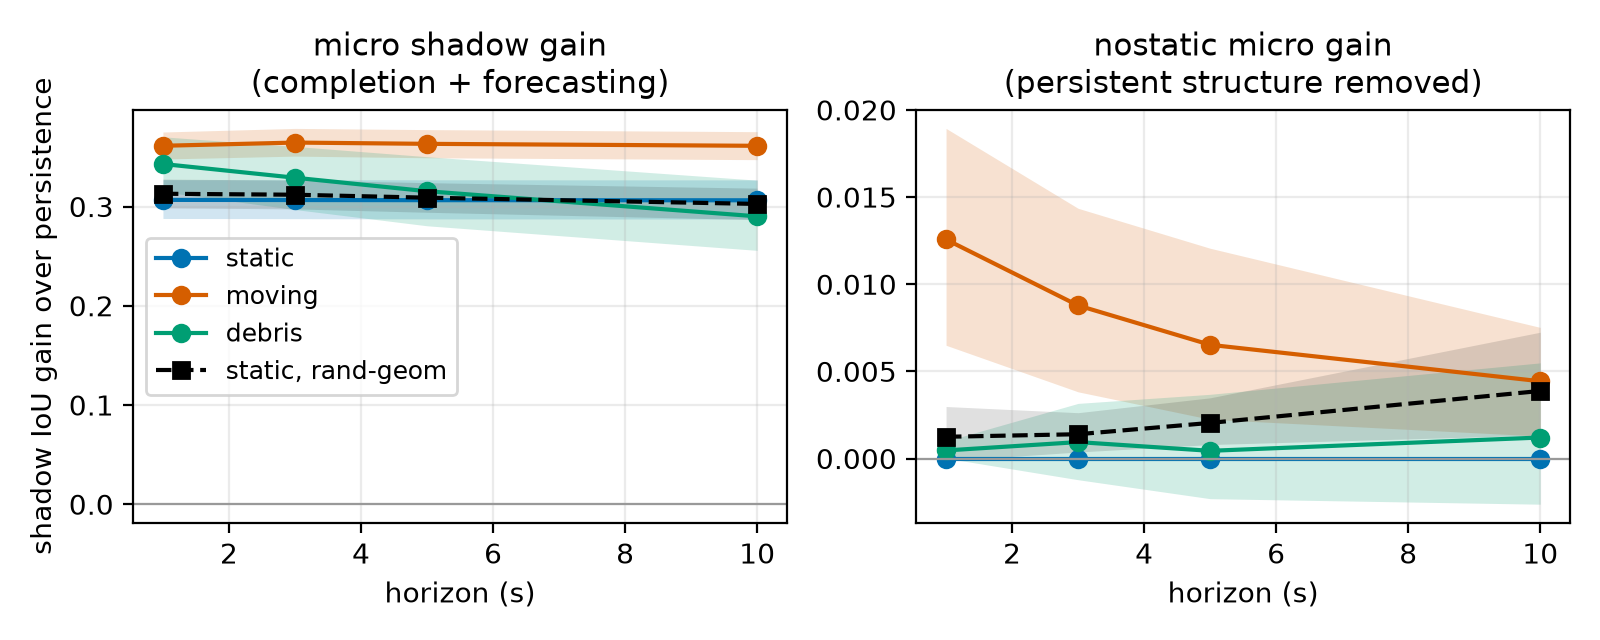
\includegraphics[width=0.8\linewidth]{shadow_gain_ci.png}
  \end{minipage}
  \caption{Micro shadow-IoU gain over persistence with 95\% per-episode bootstrap CIs: per tier
  at 5\,s, fixed geometry (left) and across horizons (right); every interval is clear of zero.}
  \label{fig:shadowgain}
  \vspace{-8pt}
\end{figure}

\textbf{Observation-blind prior.} Persistence could be a weak baseline for \emph{completion}, so
we also evaluate a pose-marginal dataset prior (mean training-set occupancy in the egocentric
frame, no observation at all), swept over thresholds and scored at its most favorable one. It reaches only 0.08--0.10 micro shadow IoU across tiers (0.09 on the
randomized-geometry set): to recall hidden structure (0.87--0.92) it must blanket 72--79\% of
genuinely empty hidden space with false positives, whereas the model achieves 0.61--0.72 IoU at
a 1.4--3.4\% false-positive rate. Completion is thus observation-conditional inference, not a
memorized average room; with geometry randomization (below), this rules out memorized layouts
and marginals alike.

\textbf{Completion, not clairvoyance.} Decomposing the shadow mask attributes the gain almost
entirely to amodal completion (Table~\ref{tab:decomp}). Excluding all persistent structure, the
residual ``nostatic'' gain sits at the noise floor: fixed static +0.000, moving +0.007 (CI
[+0.002, +0.012]), randomized-geometry static +0.002 ([+0.001, +0.004]) at 5\,s. The honest
claim is \textbf{amodal completion of hidden structure}, plus a small but statistically
significant moving-tier forecasting signal that decays with horizon as genuine forecasting
should. We do not claim dynamic forecasting on debris, where the dynamic signal is at the noise
floor and persistence matches the model beyond 1\,s.

\begin{table}[t]
  \centering
  \caption{Top: shadow-mask decomposition at 5\,s, fixed geometry (dynamic IoU spans
  1\,s$\to$10\,s): the gain is recall of persistent structure, not forecasting. Bottom:
  static-tier gain, fixed vs per-episode randomized geometry.}
  \label{tab:decomp}
  \footnotesize
  \begin{tabular}{lcc}
    \toprule
    component (fixed val @5\,s) & model & persistence \\
    \midrule
    persistent-structure recall (amodal completion) & 0.83--0.93 & 0.37--0.51 \\
    dynamic IoU, moving tier (1\,s$\to$10\,s) & 0.092 $\to$ 0.031 & 0.060 $\to$ 0.020 \\
    dynamic IoU, debris tier & 0.020 $\to$ 0.019 & 0.006 $\to$ 0.023 \\
    false-positive rate on never-occupied cells & 0.014--0.034 & 0.022--0.027 \\
    \bottomrule
  \end{tabular}\\[5pt]
  \begin{tabular}{lccc}
    \toprule
    static tier, @5\,s & micro shadow gain & 95\% CI & completion recall \\
    \midrule
    fixed $6\times6$ geometry & +0.306 & [+0.288, +0.327] & 0.829 \\
    \textbf{randomized geometry} & \textbf{+0.309} & \textbf{[+0.294, +0.324]} & 0.854 \\
    \bottomrule
  \end{tabular}
  \vspace{-6pt}
\end{table}

\textbf{Robustness to room geometry (memorization confound-kill).}
A fixed room shell could let the model memorize a constant wall prior, so we regenerated data
with per-episode random width and depth (i.i.d.\ in $[5, 8]$\,m, obstacle counts scaled to keep
${\sim}$7\% positives), retrained from scratch, and evaluated on 80
held-out randomized rooms (Table~\ref{tab:decomp}, bottom): the gain does not drop (intervals overlap almost
entirely) and completion recall is if anything higher on never-seen rooms: completion is
per-scene inference, not a memorized shell.

\textbf{Calibration in shadow.}
At 5\,s, in-shadow ECE is 0.043--0.047 across tiers --- \emph{better} than in observed space
(0.058--0.086) --- with Brier 0.022--0.036; excluding persistent structure entirely, in-shadow
ECE remains 0.055--0.056 on the tiers with dynamic content (the static tier's
structure-excluded region has no positive labels, hence no curve), so the calibration is not
carried by the easy always-occupied cells. The model is underconfident in the mid-range but
places little mass there; calibration is no fixed-room artifact: on randomized geometry,
in-shadow ECE is 0.050--0.067 vs observed 0.056--0.077, with shadow the better-calibrated
region at 5--10\,s.

\textbf{Ablations.} Retraining without either auxiliary channel leaves the gain intact:
no-visibility per-tier gains at 5\,s (+0.309/+0.360/+0.313 vs full +0.306/+0.363/+0.315) are
within CI and the no-flow rollout gain (+0.381 vs +0.320) is if anything higher; both are
redundant (no optical flow on the critical path).

\textbf{System.} The perception-to-planning path runs at 5.97\,ms p50 / 7.00\,ms p95 (batch 1,
deterministic U-Net), inside a 50\,ms (20\,Hz) budget; the excluded monocular-depth stage is
not free (Depth-Anything-V2-Small: 49.9\,ms p50 / 50.7\,ms p95 in isolation, 54.4\,ms measured
end-to-end sequential, evaluation-era GTX~1080~Ti, $480{\times}640$), so deployment runs depth
asynchronously while the 7\,ms completion path consumes the latest depth frame at 20\,Hz
(audio synthesis excluded). A falling-object \emph{proxy} (cell-level detection 0.787 at 2.62\,s mean lead;
component-level 0.752, precision only 0.714) counts events per due prediction, not per object,
keys on cells revealed rather than newly occupied (occluded static geometry revealed by agent
motion also counts), and its lead is bounded by the \{1,3,5,10\}\,s horizon grid, missing the
$\ge$3\,s target; we report it as a diagnostic, not a strength. Navigation: per-episode
collision rate 0.367 (vs 0.60 untrained; straightness 0.773), missing the $\le$0.10 target ---
an honest demonstration, no more.

\textbf{Generative variant.} A conditional-diffusion (DDPM) world model is ongoing work:
iterated DDIM sampling exceeds our batch-eval budget; a like-for-like comparison is future work.

\section{Related work}
\label{sec:related}

Predicting the structure of unobserved space has been approached from three angles. Semantic scene
completion, from SSCNet \citep{song2017sscnet} through MonoScene \citep{cao2022monoscene} and its
monocular successors VoxFormer \citep{li2023voxformer} and VisHall3D \citep{lu2025vishall3d},
infers dense voxel geometry --- and even
hallucinates geometry beyond the visible frontier --- from a single image, but targets outdoor
driving voxels evaluated purely by mIoU/IoU, without calibrated uncertainty in the occluded region.
Occupancy world models such as OccWorld \citep{zheng2024occworld}, together with occupancy-forecasting
benchmarks (Occ3D; \citealp{tian2023occ3d}) and self-supervised raycasting forecasters
\citep{khurana2023pointcloud}, instead predict the \emph{temporal} evolution of multi-frame occupancy for autonomous vehicles.
Closest in spirit, ProxMaP \citep{sharma2023proxmap} completes indoor proximal occupancy from a single
view for navigation, yet emits only point estimates. ShadowWeave is distinct: egocentric BEV amodal
completion into explicitly masked occluded space from one monocular-depth frame, with calibrated
uncertainty inside the hidden region.

\section{Conclusion and limitations}
\label{sec:conclusion}

Calibrated amodal completion of occluded occupancy works from one monocular-depth frame,
transfers to never-seen rooms, and fits a real-time perception-to-planning budget; the
empty-credit-immune micro-gain, per-episode CIs, and completion/forecasting decomposition keep
the claim honest and, we hope, get reused. The limitations are those it surfaces:
evaluation is in simulation (ground-truth occluded occupancy is unavailable on real footage
without instrumentation), so we make no quantitative real-world claim, though the front-end
already accepts real monocular depth (Depth-Anything-V2), making sim-to-real transfer the
natural next step; the model performs amodal
\emph{completion}, not multi-step \emph{forecasting}, and is framed accordingly; navigation
misses its collision target and the audio interface is not user-evaluated (system context); and
falling-object lead is bounded by the horizon grid.

\bibliographystyle{plainnat}
\bibliography{references}

\end{document}
